\section{Shamanic Interface} \label{sec:develop_interface}
    Speaking broadly, the Shamanic Interface acts as a module responsible for bridging the tasks of gesture detection and their meaningful interpretation. Towards that purpose, past work identified a number of requirements that must be met and a suggested architecture that meets them, and then followed them in implementation. One such requirement is it should have a Logic Layer that not just carries out gestures and commands as data structures, but also performs the mapping between the two. These data pairs would then in turn have an added dimension corresponding to each culture types that the system is aware of. This core component that handles the data mapping logic is called the \emph{Cultural Layer}. Booting a Shamanic interface into an application involves creating Cultural Layer and keeping it loaded until it generates the next necessary component. \\
    The input the cultural layer takes to function are a set of gesture models, a list of commands and meanings expected from them, and finally, a selected user culture. With these, it produces the Shamanic Interface’s other core component, a \emph{Classifier}. The Classifier’s purpose is to take gesture data as input, and output what command best fits the gesture performed. For all intents and purposes, the Classifier may act as an abstraction black box for the two steps of interpreting the data’s best fit with one of the internal gesture models, and then the reverse lookup between that model and the selected culture towards a given command, the latter being the output.\\
    With this architecture setup, two major points of communication between the Application’s logic and the Shamanic Interface’s logic are defined. The first is during the Shamanic Interface’s Initialization process, which occurs a single time when it loads its pre-built Gesture Model files and receives a list of commands required and a choice of culture. The other moment is a repeatable event, the Classification process, during which data is fed to the Classifier and it outputs the expected command.\\
    
    \begin{figure}[ht]
        \centering
        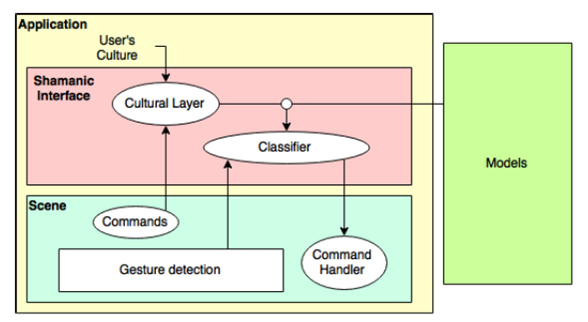
\includegraphics{figures/ShamanicBasicArchitecture.png}
        \caption{\label{fig:ShamanicBasicArchitecture}Basic Architecture of a Shamanic Interface}
    \end{figure}
    
    Previous work defined an application that followed this basic architecture. However, this operation is insufficient for the purposes of the present work’s design. One major change in the requirements is the need for multiple classifiers during completion of the game, hence, the ability for the Shamanic Interface to react to context switching, such that gestures that previously should be recognized as commands no longer should be recognized in the same manner, if at all.\\
    This is where the concept of \emph{State} is introduced. States are a smaller selection of Commands which will generate a different Classifier. Instead of being discarded from memory, the Cultural Layer is always kept in memory, ready to generate new Classifiers on demand. There’s a number of advantages to this approach. Compared to receiving commands but ignoring it at application level, there are benefits to classification accuracy in generating a classifier with only the fewer actions required. This also provides a larger degree of potential adaptability to the interface based on implementation, given that it provides a method by which the application can fall back to alternate classification. With this change, an additional stage of communication is added between the Application and the Shamanic Interface.\\
    
    \begin{figure}[ht]
        \centering
        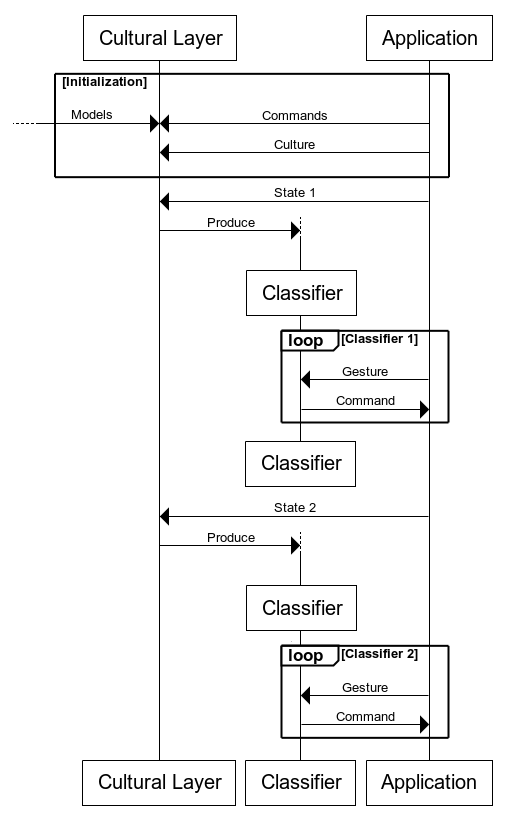
\includegraphics{figures/SequenceDiagram.png}
        \caption{\label{fig:ShamanicSequenceDiagram}Interaction Diagram for generation and usage of multiple Classifiers}
    \end{figure}

\subsection{Gesture Classification and Recording} \label{sec:develop_Classifiers}
    The method used for Gesture Classification is specific to each implementation of a Shamanic Interface. Optimally, classification and type of models used would be an entirely decoupled and independent process so the interface can be more adaptable to new solutions. Nevertheless, given the scope of the present work being very small and, while the Shamanic Interface in its state, given the separation of roles between the cultural layer and the classier, could easily be further refactored to make use of alternate models, the module employed makes use of a single gesture detection method and would require further work to generalize its model usage.\\
       
    %Pagebreak required so the image shows up here instead of several sections later.
    \clearpage
    
    As stated previously in the opening of this chapter, the models used to generate Classifiers with are built using an Accord.NET library's Hiddden Markov Learning module. The Classifier is loaded with gesture classification models based on Hidden Markov Model, in simple terms, state machines where each state has probabilistic transitions. The Classifier acts as a filter, outputting the most likely match between an input noisy set of data values (the recorded gestures) and each of the models. The filter yields matches above a threshold probability, and defaults to the neutral gesture, the first one loaded, if none of the models has a good enough fit. To achieve this setup, it was required to create, and therefore train, these gesture classification models to load the Classifiers with. Thus, the models were trained by employing an unsupervised learning algorithm called the Baum-Welch Learning Algorithm, and utilizing a Forward Topology for the Hidden Markov Models. The number of states permitted in the Model's topology is customizeable before training, with more states often resulting in higher likelihood of accurarcy, but requiring longer amount of times to produce the model. Models were trained with static tolerance, but with different levels of Forward states, starting at 6 and going up to 20, with all but the best matching model discarded and the remaining one then tested and incorporated into the shamanic interface. More information on training these models can be found on \cite{classHMMAlgorithms}.\\

    As for the recording of Gestures to produce the models with, little work was done to the prior Gesture Recorder application beyond compatibility necessary with the Shamanic Interface’s end. Sequences of Gestures are recorded using the same Leap Motion device that will later perform Gesture Detection during the game’s application. These Sequences are captured as Frames, structures detailing hand and finger directions and movement during the recording segment. A total of 200 sequences were recorded for each gesture and each hand, to be used as training data for the models (4000 samples spread accross 20 classes).
